\documentclass[10pt, a4paper]{article}

\usepackage[top=1.2cm, bottom=1.8cm, left=1.5cm, right=1.5cm]{geometry}
\usepackage{hyperref}
\usepackage{enumitem}
\usepackage{titlesec}
\usepackage{fontenc}
\usepackage{inputenc}
\usepackage{parskip}
\usepackage{xcolor}
\usepackage{graphicx}
\usepackage{fancyhdr}
\usepackage{eso-pic}

\hypersetup{
    colorlinks=false,
    allbordercolors=black,
    pdfborderstyle={/S/U/W 1}
}

% Section formatting
\titleformat{\section}{\large\bfseries}{}{0em}{}[\titlerule]
\titlespacing{\section}{0pt}{6pt}{4pt}

\setlist[itemize]{noitemsep, topsep=2pt, leftmargin=1.2em}

% Footer
\pagestyle{fancy}
\fancyhf{}
\renewcommand{\headrulewidth}{0pt}
\fancyfoot[C]{\small The updated version of this document is available at \href{https://adityamitra5102.github.io/resume-short.pdf}{\underline{https://adityamitra5102.github.io/resume-short.pdf}}}

% QR code bottom right on every page
\AddToShipoutPictureBG{%
  \AtPageLowerLeft{%
    \hspace{\dimexpr\paperwidth-2.0cm\relax}%
    \raisebox{0.3cm}{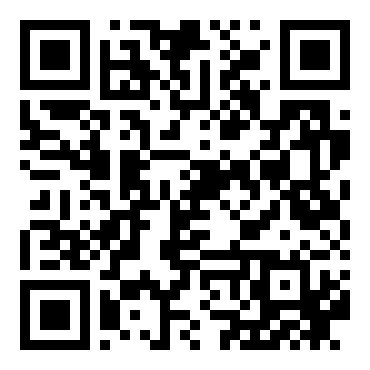
\includegraphics[width=1.5cm]{qrcode.png}}%
  }%
}

\begin{document}

% ── HEADER ──────────────────────────────────────────────────────────────────
\begin{center}
    {\LARGE\bfseries Aditya Mitra}\\[4pt]
    {\small Cybersecurity Researcher · Security Engineer · FIDO2/Passkeys Specialist}\\[4pt]
    {\small
        \href{mailto:adityamitra5102@gmail.com}{\underline{adityamitra5102@gmail.com}} ·
        \href{https://www.linkedin.com/in/AdityaMitra5102}{\underline{LinkedIn}} ·
        \href{https://adityamitra5102.github.io}{\underline{Website}} ·
        \href{https://scholar.google.com/citations?user=oXPSCNUAAAAJ}{\underline{Google Scholar}} ·
        \href{https://orcid.org/0000-0002-9612-0810}{\underline{ORCID}} ·
        \href{https://www.credly.com/users/aditya-mitra.a830b75a/badges}{\underline{Credly}}
    }
\end{center}

\vspace{4pt}

% ── INTRO ───────────────────────────────────────────────────────────────────
\noindent
I make secure systems. I make systems secure. My work spans passwordless authentication, applied cryptography, and systems security --- from the first physical FIDO2 security key with post-quantum cryptography to enterprise authentication infrastructure and open-source security tooling. Erasmus Mundus Scholar in Applied Cybersecurity, active researcher with 15+ publications across IEEE, Springer, and Elsevier, and currently contributing to Nitrokey GmbH's security stack.

% ── EDUCATION ───────────────────────────────────────────────────────────────
\section*{Education}

\noindent\textbf{M.Sc. in Cybersecurity} · Erasmus Mundus Joint Masters (CyberMACS) · 2025 -- Present\\
Kadir Has University, Istanbul, Turkey\\
\textit{Erasmus Mundus Scholar}

\vspace{4pt}

\noindent\textbf{B.Tech. in Computer Science and Engineering} (Specialization: Robotics) · CGPA: 8.32 · 2020 -- 2024\\
VIT-AP University, Andhra Pradesh, India

% ── EXPERIENCE ──────────────────────────────────────────────────────────────
\section*{Experience}

\noindent\textbf{Software Development Intern} · Nitrokey GmbH · June 2026 -- Present
\begin{itemize}
    \item Development of Nitrokey 3 management software.
\end{itemize}

\vspace{4pt}

\noindent\textbf{CTO} · Digital Fortress Pvt. Ltd. · January 2023 -- Present
\begin{itemize}
    \item Architected and built a passwordless authentication backend from scratch in under 3 days, deployed at enterprise scale with SSO and CSP capabilities.
    \item Led a team of 7 engineers building next-generation FIDO2-based authentication systems.
    \item Deployed and maintained cloud infrastructure across Azure and Linux-based on-premises servers.
\end{itemize}

\vspace{4pt}

\noindent\textbf{Researcher} · Center of Excellence in AI and Robotics, VIT-AP · February 2022 -- Present
\begin{itemize}
    \item Researching passwordless authentication, FIDO2/passkeys, post-quantum cryptography, and IoT security.
    \item 15+ publications across IEEE, Springer, Elsevier, and arXiv.
\end{itemize}

\vspace{4pt}

\noindent\textbf{Pentester Intern} · Fresh Digital · March 2022 -- April 2022
\begin{itemize}
    \item Conducted penetration testing of production environments; identified compliance gaps and delivered remediation strategies.
\end{itemize}

% ── RESEARCH INTERESTS ──────────────────────────────────────────────────────
\section*{Research Interests}

\noindent FIDO2 / Passkeys · Post-Quantum Cryptography · Passwordless Authentication · Cryptographic Protocols · Protocol Design · Systems Security · IoT Security · Networking · Decentralized Identity

% ── SKILLS ──────────────────────────────────────────────────────────────────
\section*{Skills}

\noindent\textbf{Languages \& Tools:} Python, C, Java, Bash, Git, Linux, CUDA\\
\textbf{Cryptography \& Security:} Cryptographic protocol design, FIDO2/WebAuthn, Post-Quantum Cryptography, PKI, ISO 7816\\
\textbf{Platforms \& Infra:} Linux, bare-metal deployment, on-premises infrastructure, networking, Azure, SQL\\
\textbf{Libraries:} Flask, python-fido2, pycryptodome, cbor2

% ── NOTABLE ACHIEVEMENTS ────────────────────────────────────────────────────
\section*{Notable Achievements}

\begin{itemize}
    \item \textbf{Vulnerability 1721, FIDO Alliance} --- Reported NFC-based MITM attack affecting all NFC FIDO authenticators
    \item \textbf{FIDO Developer Challenge India 2022, Top 3} --- FIDO Alliance organized global competition for developers building on FIDO2 specifications
    \item \textbf{Peer Reviewer} --- IEEE Access (2 papers), IEEE ICECET 2024, Elsevier Cyber Security and Applications, Springer Telecommunication Systems (2 papers), Springer Nature Computer Science
    \item \textbf{Hackathon Mentor} --- Status Code 1 (IIIT Kalyani $\times$ IISER Kolkata), FrostHacks 1.0 (Academy of Technology), HexaFalls 1.0 (JIS University)
    \item \textbf{Vice President}, Null Chapter VIT-AP (2022--2023) --- organized CTF events, security workshops, FIDO2 demos; awarded Best Member 2021--22
\end{itemize}

% ── SELECTED PROJECTS ───────────────────────────────────────────────────────
\section*{Selected Projects}

\noindent\textbf{Mariana's Qubit} \textit{(Ongoing)} · \href{https://adityamitra5102.github.io/Marianas-Qubit}{\underline{read more}}\\
Open-source, anonymous, decentralized internet stack that redefines the OSI model with privacy and censorship resistance as first principles.

\vspace{4pt}

\noindent\textbf{PQC FIDO2 Security Key} · \href{https://github.com/AdityaMitra5102/RPi-PQC-FIDO-Key-Pin-support-ecdh}{\underline{read more}}\\
First known implementation of a fully functional physical FIDO2 security key with post-quantum cryptography, built on Raspberry Pi and tested against Google, Windows Hello, and Apple.

\vspace{4pt}

\noindent\textbf{PQRSTUV -- Open Source HSM} · \href{https://github.com/AdityaMitra5102/PQRSTUV-Docs}{\underline{read more}}\\
Consumer-grade hardware HSM with post-quantum cryptographic guarantees, custom communication protocols, and IETF-aligned standards documentation.

\vspace{4pt}

\noindent\textbf{Loki} \textit{(Published in IEEE Access)} · \href{https://adityamitra5102.github.io/blog/loki.html}{\underline{read more}}\\
FIDO2-compliant physical lock for protecting physical assets using RSA and cloud security --- among the first physical locks with seamless high-security FIDO2 access control.

% ── HACKATHONS ──────────────────────────────────────────────────────────────
\section*{Hackathons \& Competitions}

\noindent Smart India Hackathon 2022 (Winner) · Microsoft Imagine Cup 2022 (India Runner-up) · INEX 2022 (Silver) · ACM ICPC 2021 (Regionalist) · ION\textless athon\textgreater~1.0 (Top 10) · Hackerearth Hack to Enable 2021 (6th)

% ── CERTIFICATIONS ──────────────────────────────────────────────────────────
\section*{Certifications}

\noindent Cisco Certified Cybersecurity Associate (CCNA Cybersecurity), Cisco Certified Network Associate (CCNA), CompTIA SecurityX (CASP+), CompTIA CySA+, CompTIA Security+, CompTIA Network+, Microsoft SC-900, Microsoft AZ-900, Oracle Java SE 8 OCA, CLA (C Programmer) · \href{https://www.credly.com/users/aditya-mitra.a830b75a/badges}{\underline{All badges on Credly}}

% ── PUBLICATIONS ────────────────────────────────────────────────────────────
\section*{Publications}

\noindent\textit{15+ total --- selected below. Full list on \href{https://scholar.google.com/citations?user=oXPSCNUAAAAJ}{\underline{Google Scholar}}.}

\vspace{4pt}

\begin{itemize}
    \item Mitra, A. et al. \textbf{Blind Eye: Motion and Obstacle Detection Leveraging Wi-Fi.} IEEE AVSS 2025, pp.~1--7. \href{https://doi.org/10.1109/AVSS65446.2025.11149826}{\underline{10.1109/AVSS65446.2025.11149826}}

    \item Mitra, A. \& Ghosh, A. \textbf{FIDO2: A Comprehensive Study on Passwordless Authentication.} IJERA 14(7), pp.~58--63, 2024. \href{https://doi.org/10.9790/9622-14075863}{\underline{10.9790/9622-14075863}}

    \item Mitra, A. et al. \textbf{/dev/SDB: Software Defined Boot.} arXiv, 2026. \textit{(Accepted \& Presented, IEEE CIIT 2023)} \href{https://doi.org/10.48550/arXiv.2601.20629}{\underline{10.48550/arXiv.2601.20629}}

    \item Mitra, A. \& Sethuraman, S.\,C. \textbf{Verifiable Passkey: The Decentralized Authentication Standard.} arXiv, 2025. \textit{(Accepted \& Presented, IEEE CIIT 2023)} \href{https://doi.org/10.48550/ARXIV.2512.21663}{\underline{10.48550/ARXIV.2512.21663}}

    \item Mitra, A. \& Sethuraman, S.\,C. \textbf{The Qey: PQC in FIDO2.} arXiv, 2025. \href{https://doi.org/10.48550/ARXIV.2510.21353}{\underline{10.48550/ARXIV.2510.21353}}

    \item Sethuraman, S.\,C., Mitra, A. et al. \textbf{Loki: FIDO2 IoT Lock for Physical Asset Security.} IEEE Access, 2022. \href{https://doi.org/10.1109/ACCESS.2022.3216665}{\underline{10.1109/ACCESS.2022.3216665}}

    \item Sethuraman, S.\,C., Mitra, A. et al. \textbf{TUSH-Key: Transferable User Secrets on Hardware Key.} IEEE ICPADS 2024, pp.~176--185. \href{https://doi.org/10.1109/ICPADS63350.2024.00032}{\underline{10.1109/ICPADS63350.2024.00032}}

    \item Ghosh, A., Mitra, A. et al. \textbf{Saila: HID Injection Protection with Smartphone-based Passwordless Security.} IEEE ICDCSW 2024, pp.~122--127. \href{https://doi.org/10.1109/ICDCSW63686.2024.00023}{\underline{10.1109/ICDCSW63686.2024.00023}}

    \item Cherukuri, A.\,K., Shaw, R., Ghosh, A., Mitra, A. et al. \textbf{FIDO2 Smart Medical Card for Healthcare.} Int.\ J.\ Critical Computer-Based Systems, 11(1/2), 2024. \href{https://doi.org/10.1504/ijccbs.2024.10064420}{\underline{10.1504/ijccbs.2024.10064420}}
\end{itemize}

\end{document}
